\section{Visibility graphs {\bf{(Yong)}}}
	\subsection{Historical roots}
In the last about 10 years, there has been a growing body of literature aiming
at the utilization of complex network methods for the characterization of
dynamical systems based on time series. While both nonlinear time series
analysis and complex network theory are widely considered to be established
fields of complex systems sciences with strong links to Nonlinear Dynamics and
Statistical Physics, the thorough combination of both approaches has become an
active field of research during the last decade, which has allowed addressing
fundamental questions regarding the structural organization of nonlinear
dynamics as well as the successful treatment of a variety of applications from a
broad range of disciplines.

With its three main concepts, phase space / recurrence networks, visibility
graphs and transition / Markov chain networks having made their way from
abstract concepts to widely used methodologies, the field of time series
networks has become mature. These three concepts, as well as several variants
thereof, have been studied in great detail regarding their specific properties,
potentials and limitations and provided fundamental new insights into the
dynamics of complex systems. In addition, these approaches have already found a
wide range of applications from such diverse fields as climatology,
neurophysiology and economics, to mention only a few examples, demonstrating the
great potentials of time series networks to tackling real-world contemporary
scientific problems.

To this end, there exists no thorough overview paper covering all existing
approaches of time series networks. Consequently, we believe that the time is
ripe to deliver such a review covering the methodological foundations,
interpretation and (potential) applications of the existing zoo of methods from
this field. We are confident that Physics Reports would be an excellent forum
for the first review that integrates the state of research on all corresponding
concepts that exist so far.

	\subsection{Algorithmic variants}
		\subsubsection{Standard visibility graphs}
		\subsubsection{Horizontal visibility graphs}
			\begin{figure}
			  \centering
			  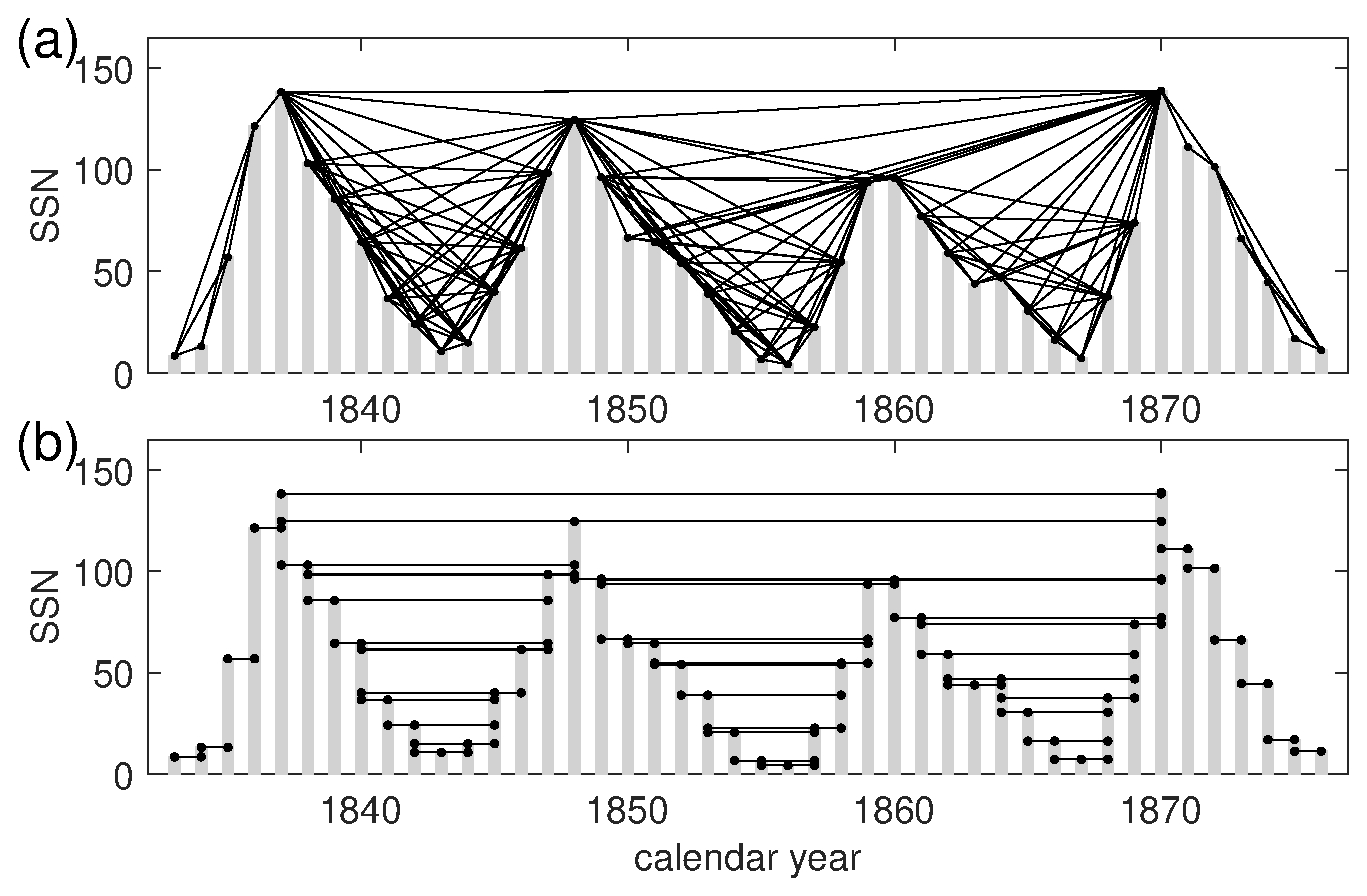
\includegraphics[width=\columnwidth]{Chapter04_VisibilityGt/TSspotnumberYear.eps}
			  \caption{Algorithm of constructing visibility graphs. \label{fig_chap04:timeseriesSS}}
			\end{figure}

	\subsection{Visibility graph properties}
		\subsubsection{Degree distributions}
		relationship with Hurst exponent in fractal / multifractal time series
		\subsubsection{Stochastic vs. deterministic dynamics}
		\subsubsection{Local network properties}
		\subsubsection{Global network properties}
		\subsubsection{Properties related to edge lengths}
		\subsubsection{Finite-sample effects}

influence of noise, missing values, time-scale uncertainty

also discuss here VGs for (marked) point processes like application to
earthquakes (Telesca et al.), draw link to natural time analysis method here???   

Maybe that's more like a separate subsection on "practical considerations",
together with noise effects, etc.

General question: What information can be gained from VGs? Which networks
properties are (when) useful to study? 

	\subsection{Bivariate visibility graph methods}
		\subsubsection{Visibility graph similarity}
		\subsubsection{Joint and excess degrees}


	\subsection{Decomposition of visibility graphs}
		\subsubsection{Time-directed visibility graphs}
		\subsubsection{Tests for time series irreversibility}
	\subsection{{\color{red} Identifying transitions by visibility graph method?
	Any references?}}
